% !TEX encoding = UTF-8
% !TEX TS-program = pdflatex
% !TEX root = ../Tesi.tex
% !TEX spellcheck = en-EN

%************************************************
\chapter{Sinter Segregator}
\label{cap:sintersegregator}
%************************************************

\section{Sinter chute design}
\label{sec:sinterchutedesign}

The method previously explained allowed to collect data regarding the contact
law. We took the average value for each of the DEM parameter and we used them 
in an industrial scale DEM simulation, with the same software, 
of an iron ore sintering process. 
Especially, we examined the behaviour of these particles in a sinter chute cooler. 
The particles moved from the top of a specifically designed chute and were 
collected by moving boxes at the bottom. These boxes were holed at the base, 
allowing cool air to lower the temperature of the sinter. 
It was critical to ascertain if the larger particles segregated, 
by moving to the bottom of the boxes, while the smaller to the top, allowing a 
more effective distribution of the cool air. The simulation was performed 
with a maximum of 500,000 particles.

\section{Sinter chute results}
\label{sec:sinterchuteresults}


There are two main phases:
\begin{itemize}
  \item{Initial filling: during this phase many small particles deposited inside
  the chute}
  \item{Moving bottom box: also in this phase particles were
continuously inserted from the top. After the filling was completed, the
scraper was moved and all the particles further a defined surface were
deleted. Inside the sinter, all the places that small particles could
occupy already were. At this point the bottom box was filled again, but
with a more realistic size distribution, and it reached steady state, as can
be seen in figures \ref{fig:043rS1}, \ref{fig:044rS2}, \ref{fig:045rS4}, and
\ref{fig:046rS6}.}
\end{itemize}
As expected, when the steady state was reached, the particles actually
segregated, as it was intended to demonstrate.
In fact, there were more particles with larger radiuses, from 8 to 25 mm, in the
bottom layers.
Instead, the smallest particles, radius = 2.5 mm, was rather on the top layer. 
\begin{figure}%[!htb] 
\centering 
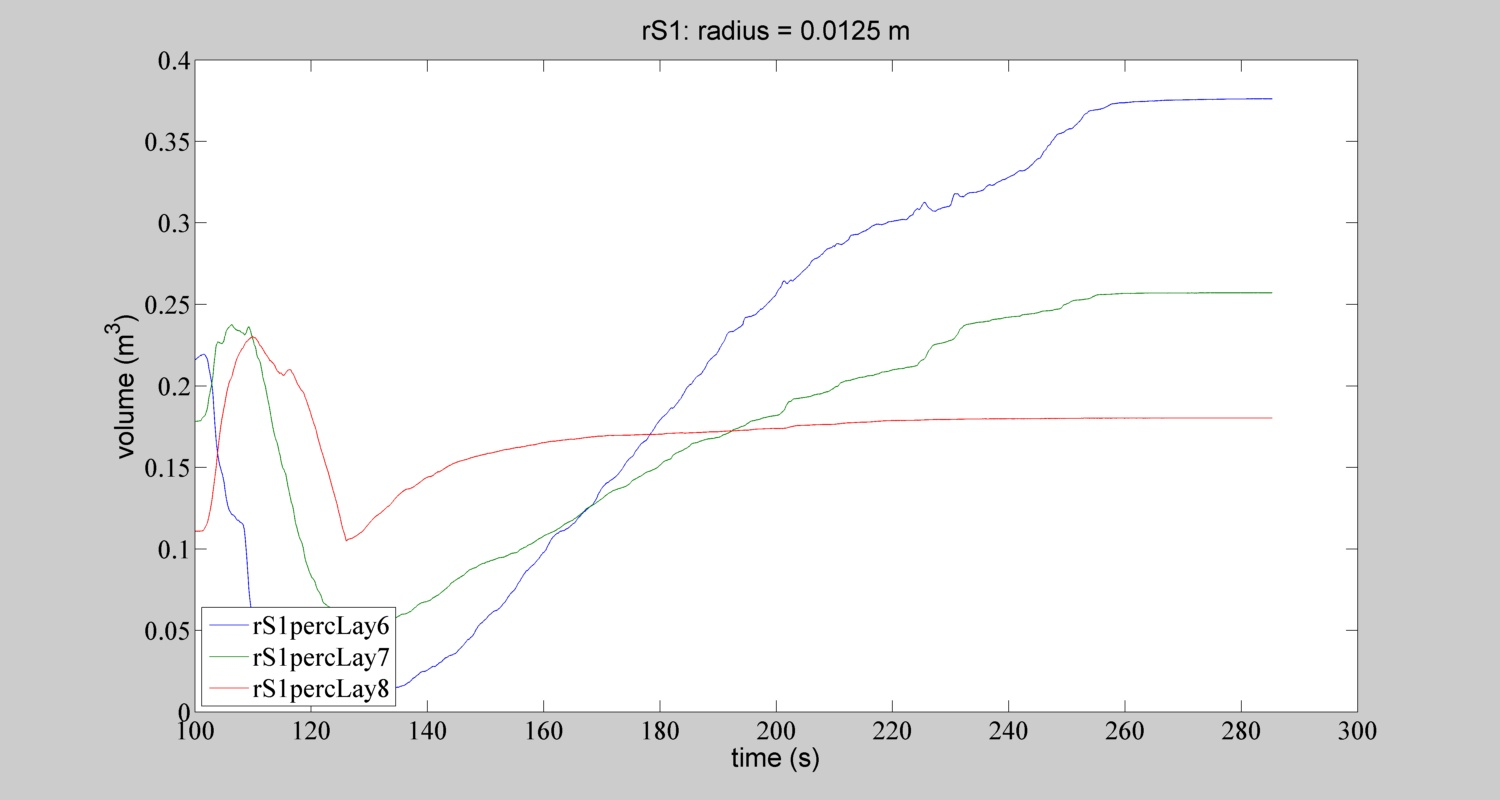
\includegraphics[width=.48\columnwidth]{images/043rS1} 
\caption{Radius 1}
\label{fig:043rS1} 
\end{figure}
%************************************************
\begin{figure}%[!htb] 
\centering 
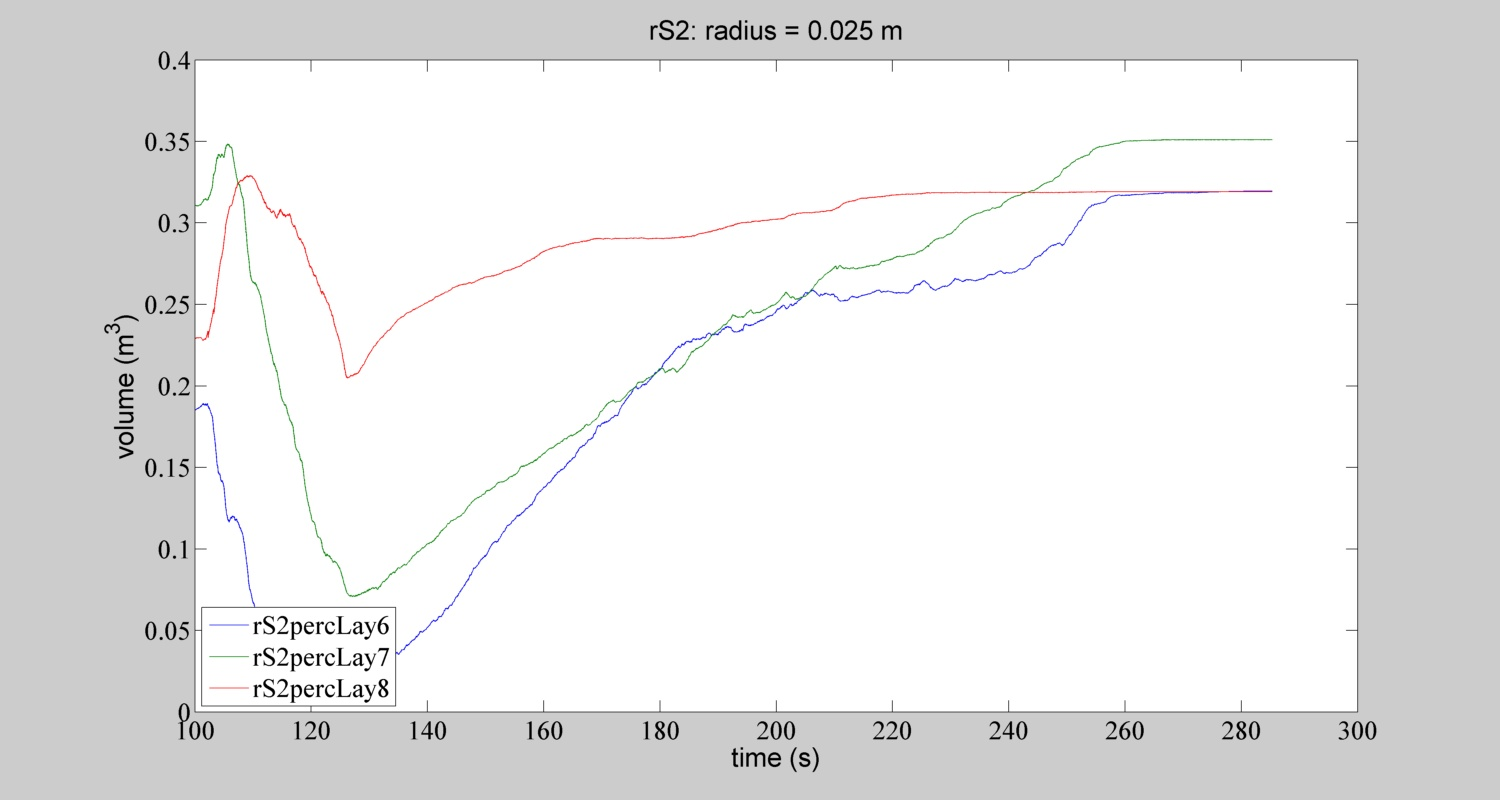
\includegraphics[width=.48\columnwidth]{images/044rS2} 
\caption{Radius 2}
\label{fig:044rS2} 
\end{figure}
%************************************************
\begin{figure}%[!htb] 
\centering 
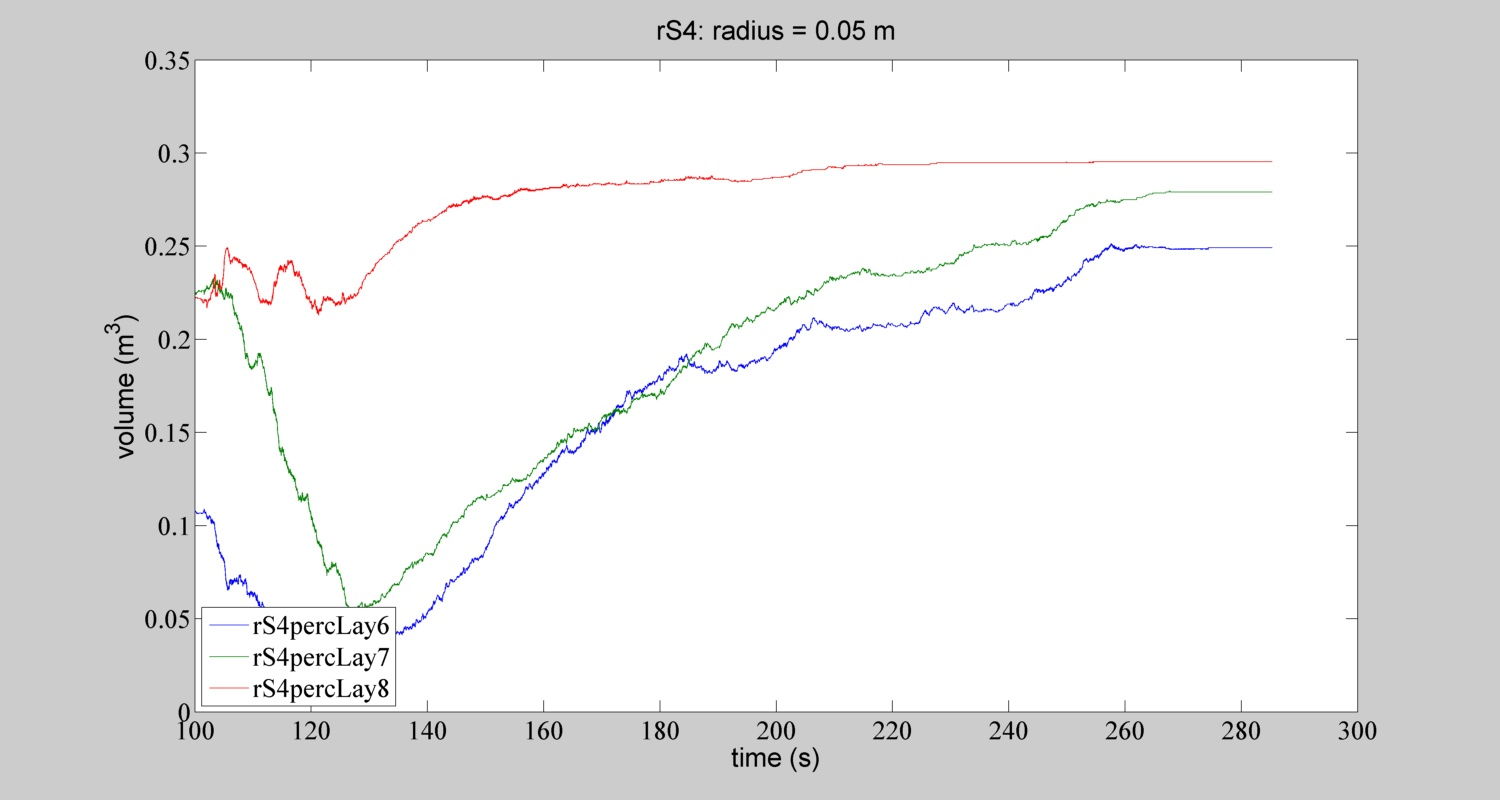
\includegraphics[width=.48\columnwidth]{images/045rS4}
\caption{Radius 4}
\label{fig:045rS4} 
\end{figure}
%************************************************
\begin{figure}%[!htb] 
\centering 
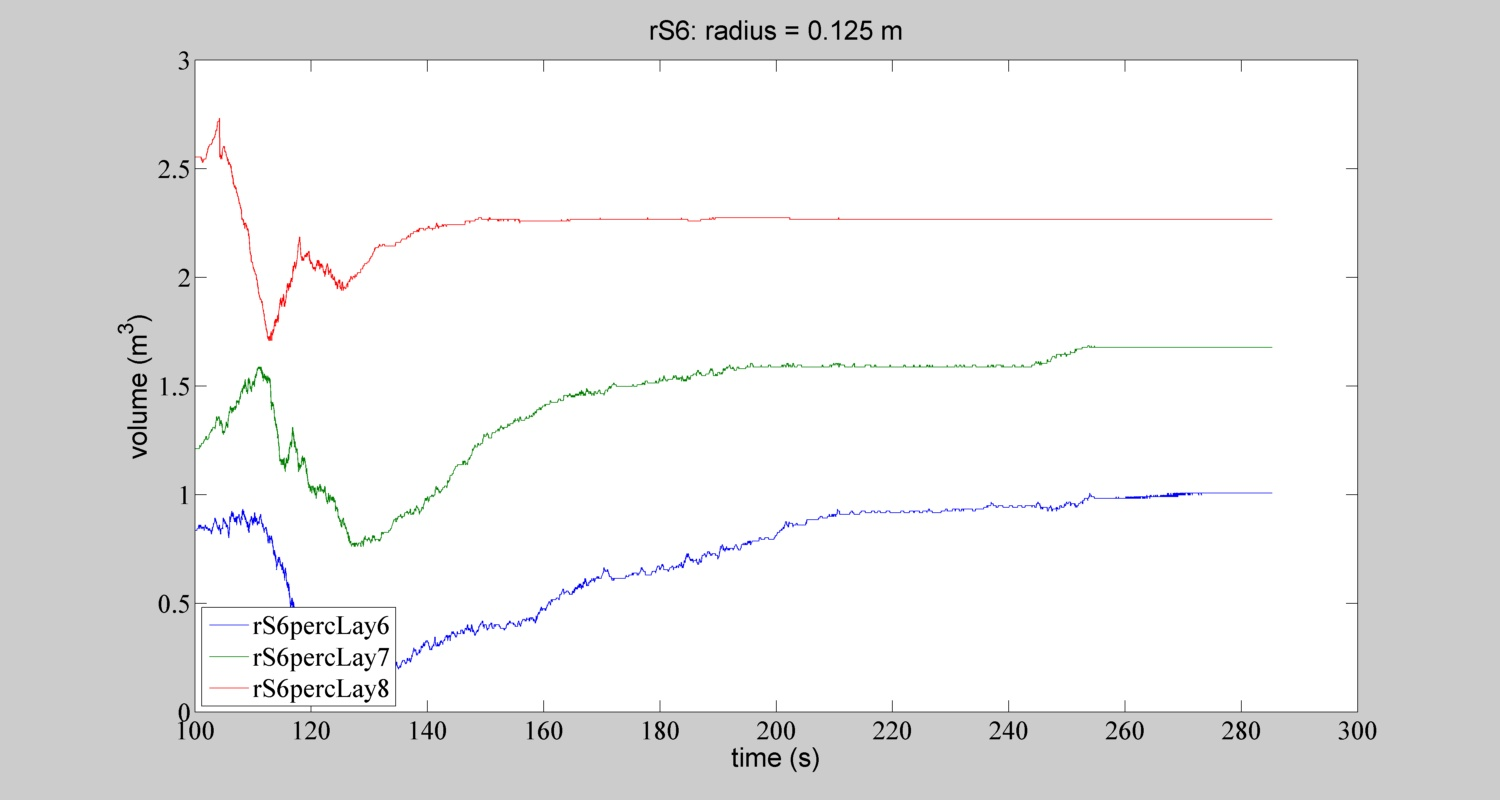
\includegraphics[width=.48\columnwidth]{images/046rS6} 
\caption{Radius 6}
\label{fig:046rS6} 
\end{figure}

As explained in the Application section, we divided the first of the boxes
filled by the chute in three (equally high) layers, from 6 on top to 8 
on bottom, see Fig. \ref{fig:056sinterChuteBox}. 
The volume over these layers was not considered, because it was continuously 
supplied of particles from the chute. In Fig. \ref{fig:066sinterbarplot} the
percentage of the total volume of the particles available in each layer at steady-state, 
grouped by radius, is shown. 
We could clearly see how the larger particles disposed mostly 
in the bottom layer, validating the realized design.


\begin{figure}[!htb]
\centering
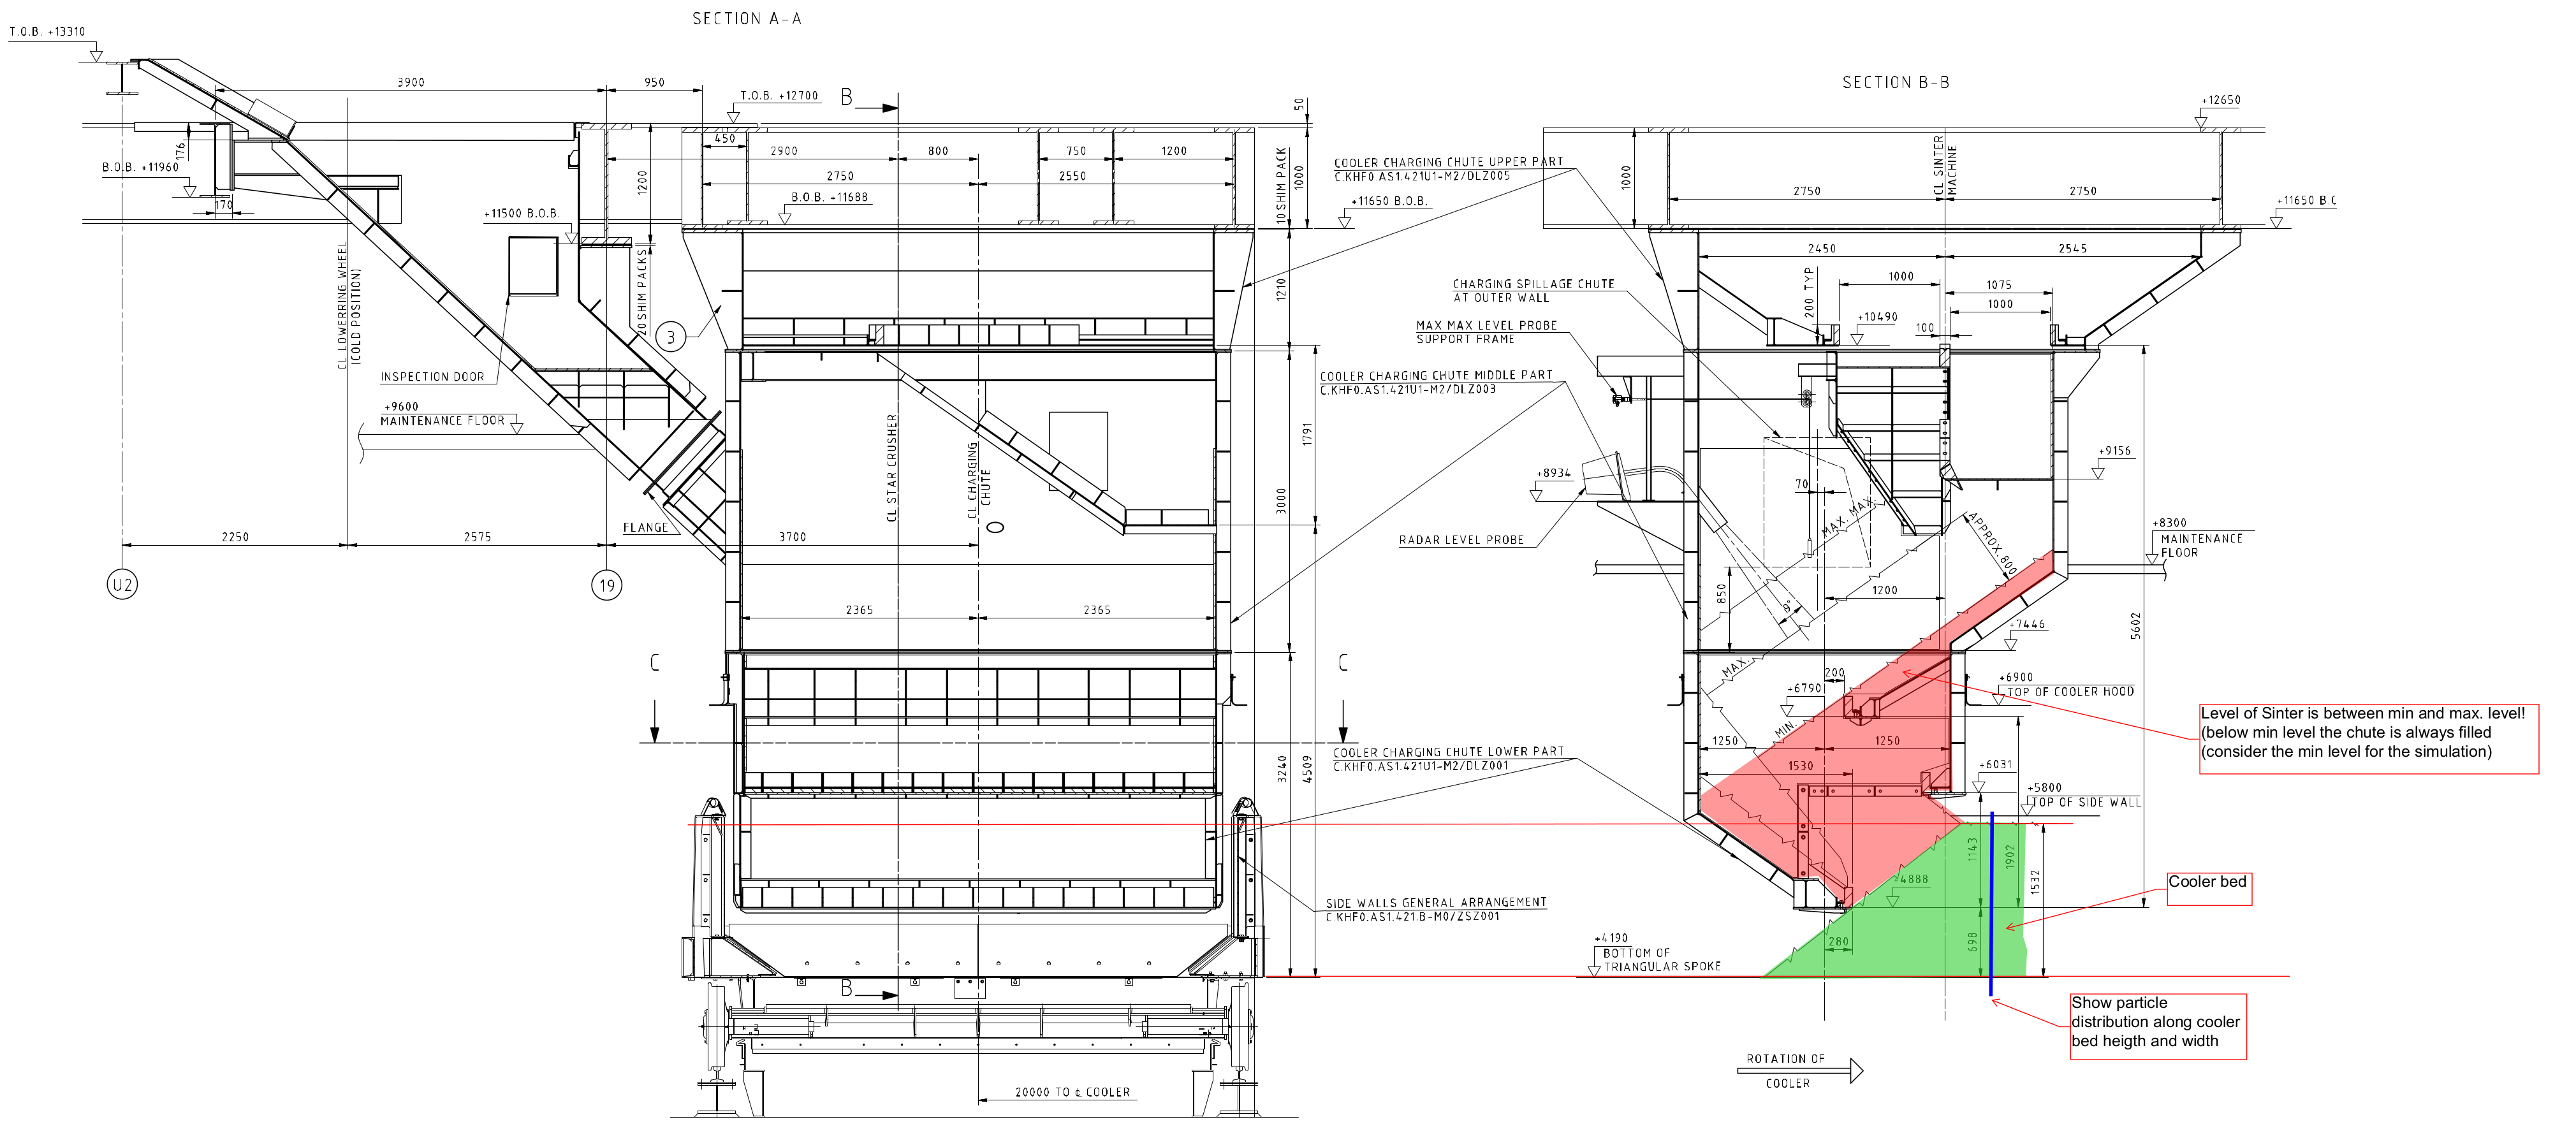
\includegraphics[width=.80\columnwidth]{055sinterChuteVerticalLayout}
\caption[Sinter chute vertical layout]{Sinter chute vertical layout.}
\label{fig:055sinterChuteVerticalLayout}
\end{figure}
\ref{fig:055sinterChuteVerticalLayout} \\

\begin{figure}[!htb]
\centering
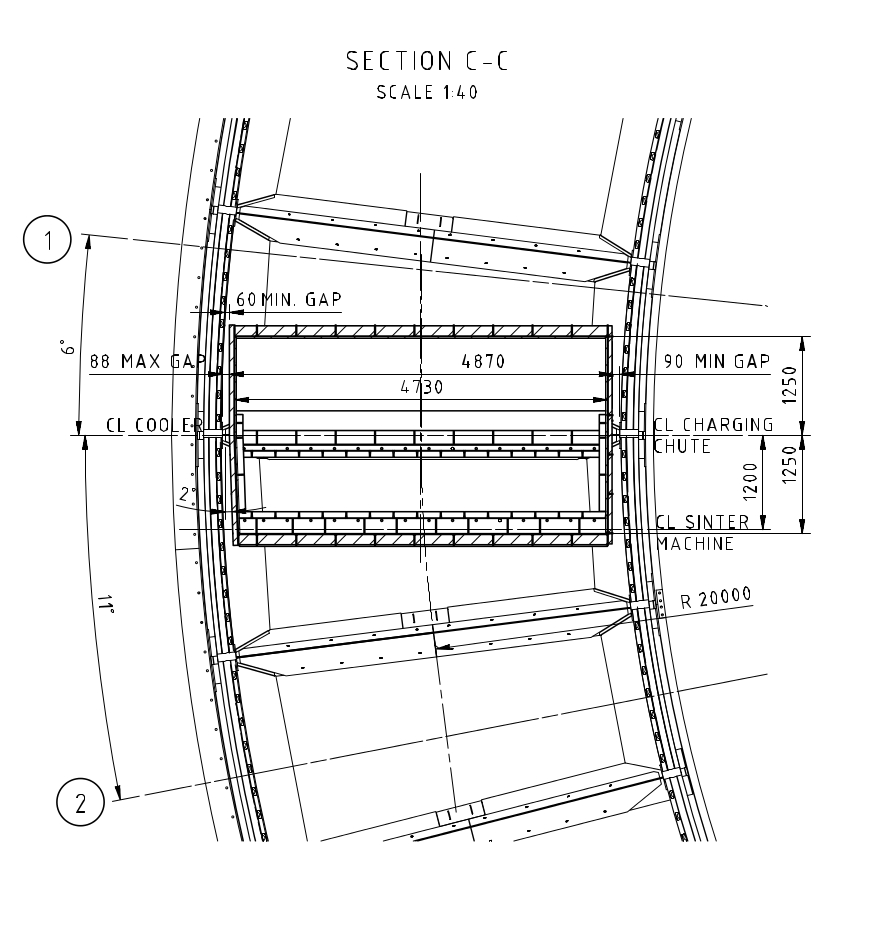
\includegraphics[width=.80\columnwidth]{images/056sinterChuteBox}
\caption[Sinter chute box]{Sinter chute box (Primetals GmbH).}
\label{fig:056sinterChuteBox}
\end{figure}


\begin{figure}[!htb]
\centering
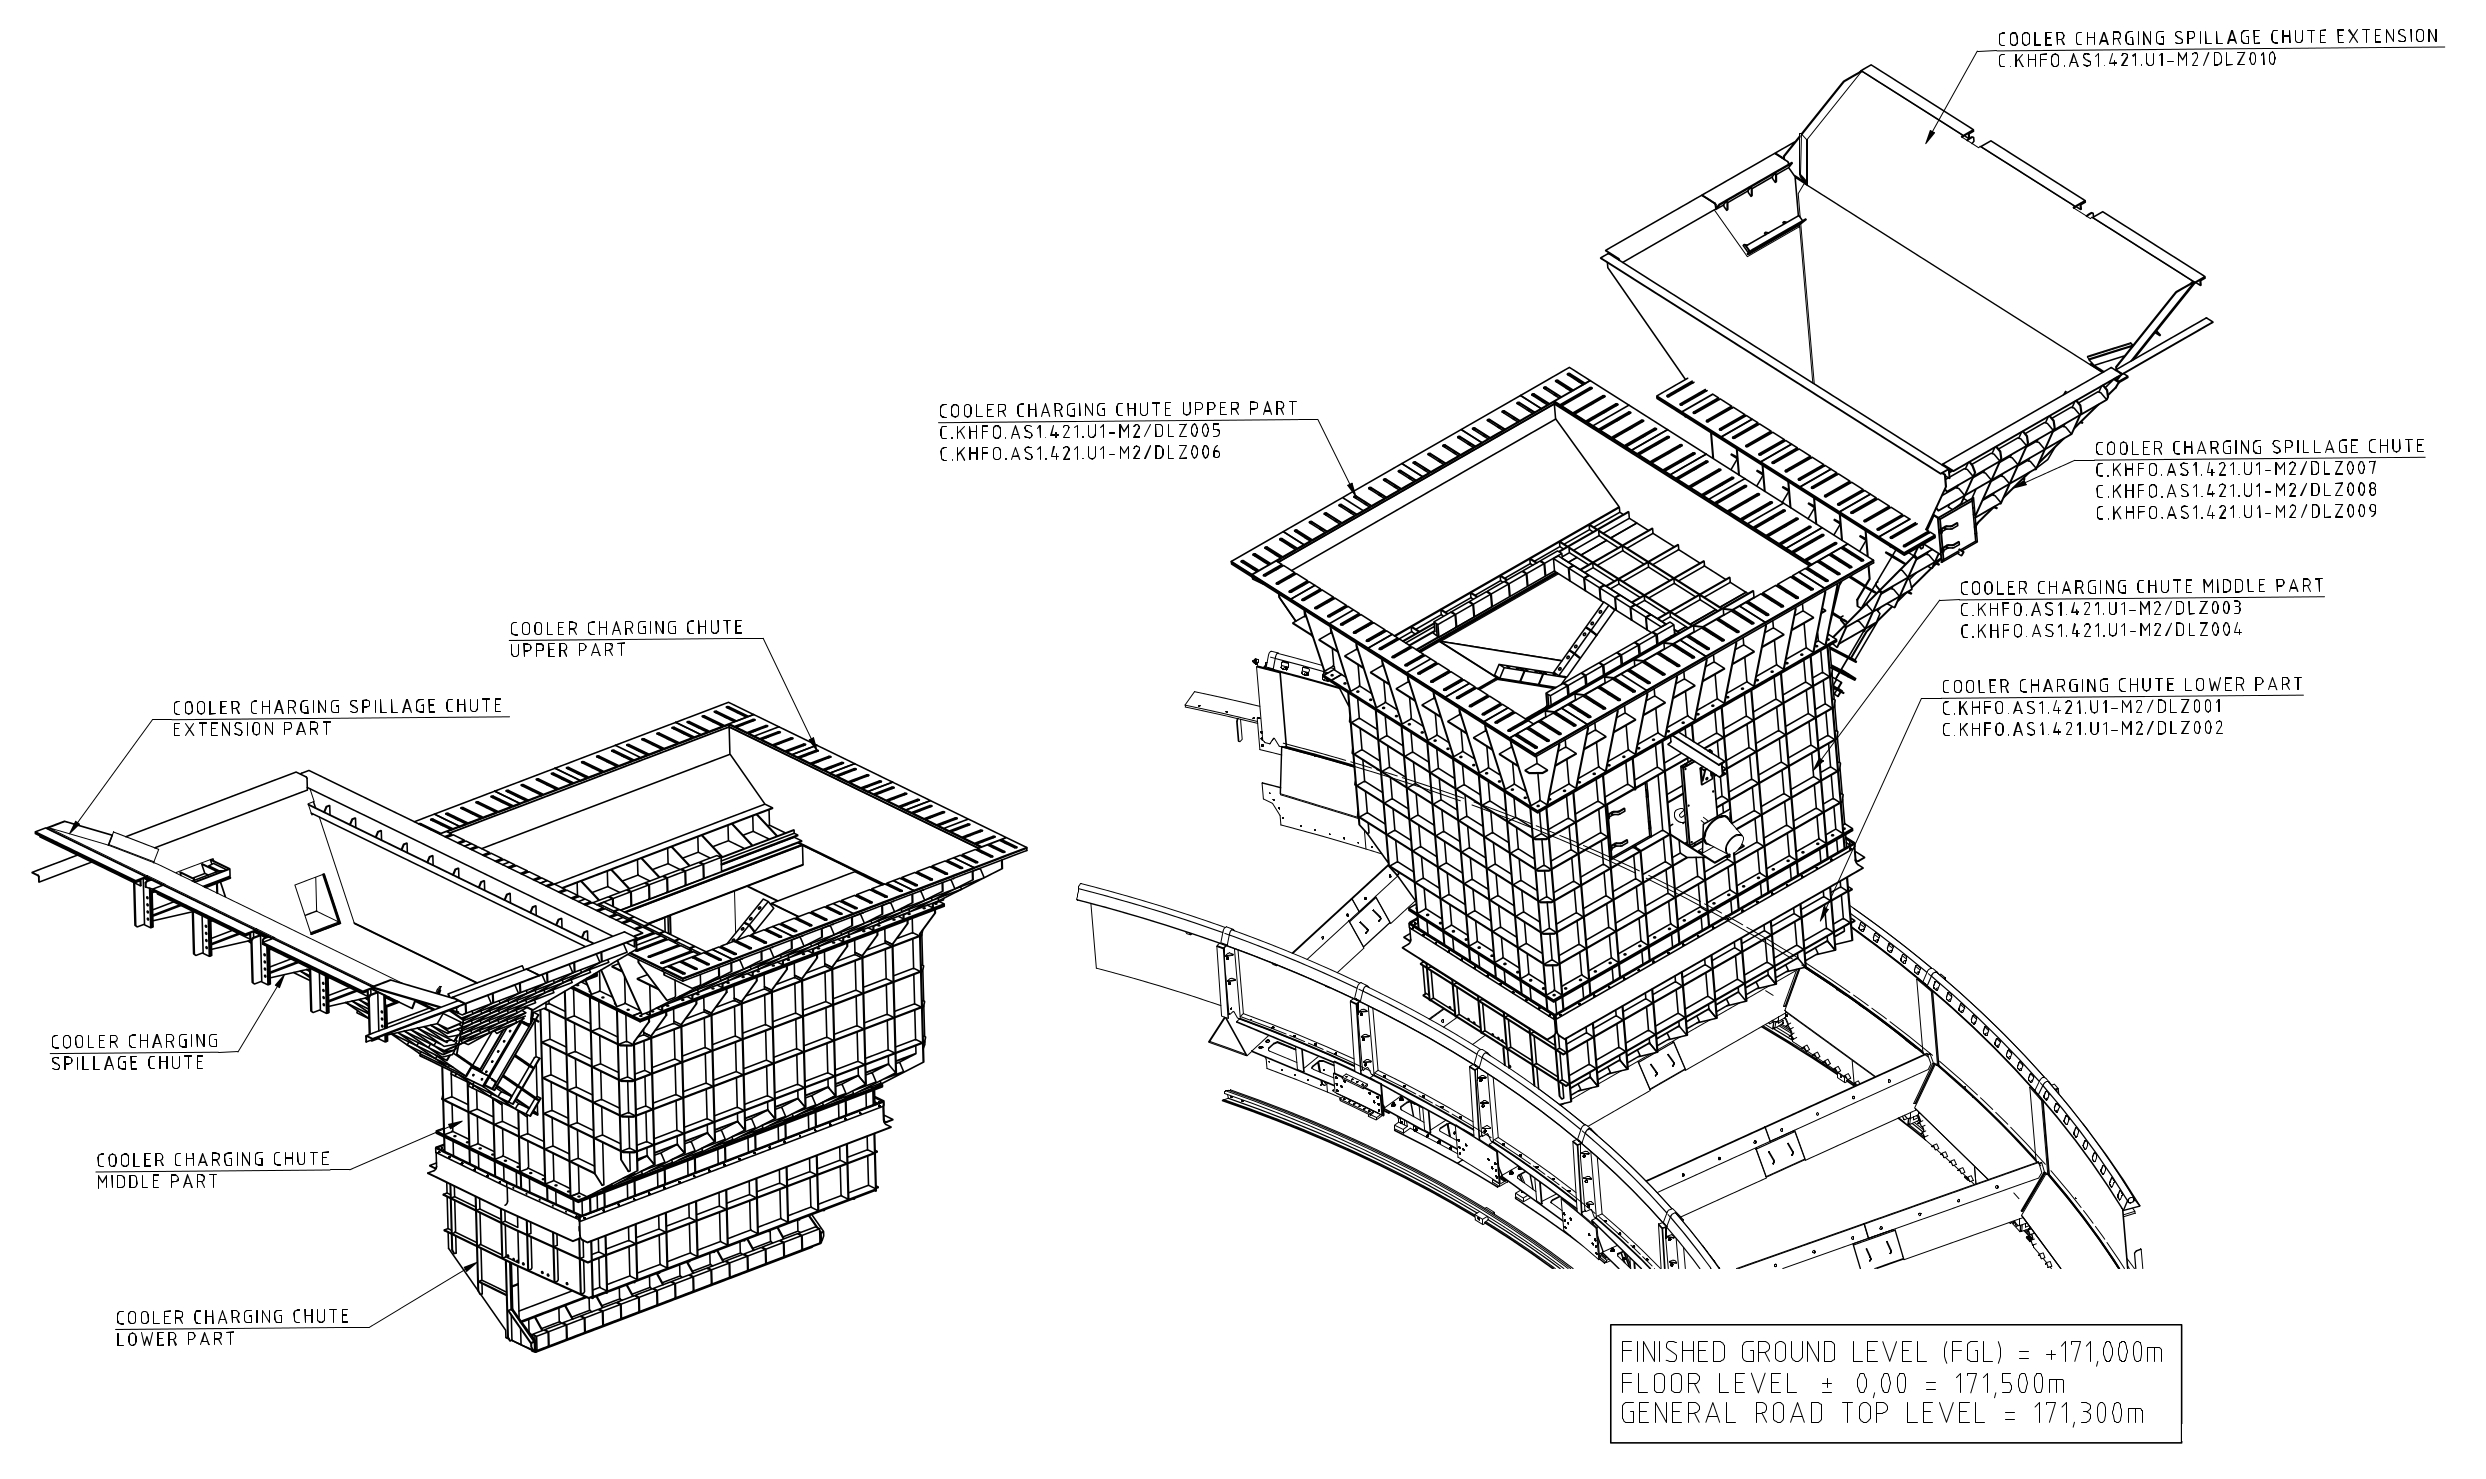
\includegraphics[width=.80\columnwidth]{images/057sinterChuteOrtoLayout}
\caption[Sinter chute orto layout]{Sinter chute orto layout.}
\label{fig:057sinterChuteOrtoLayout}
\end{figure}
\ref{fig:057sinterChuteOrtoLayout} \\

\begin{figure}[htbp]
\centering 
  \subfloat[Ratio over the volume occupied by the particles of each radius.]
  {
	  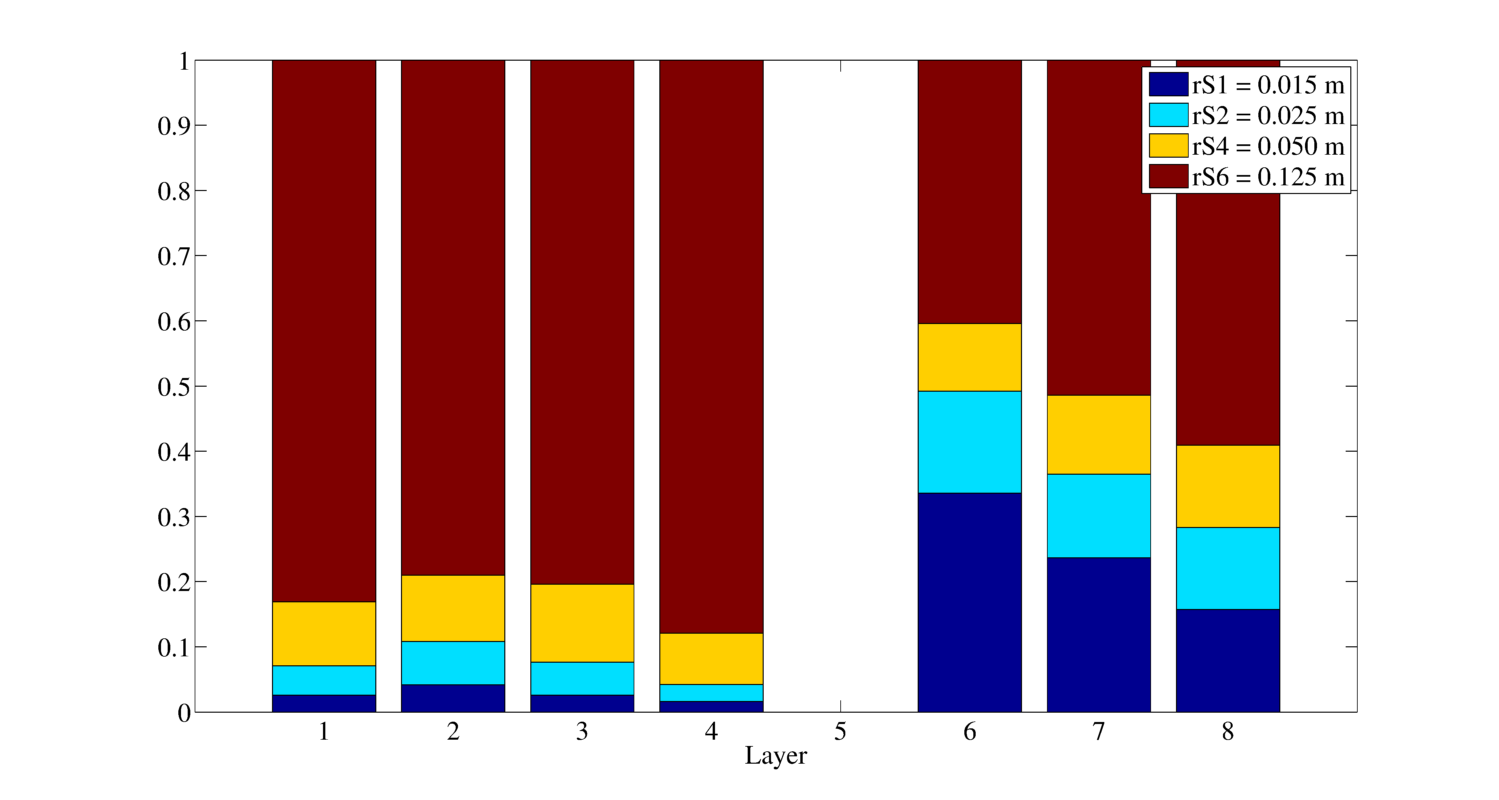
\includegraphics[width=.96\columnwidth]{images/121SinterBarPlot20151111150702}
	  \label{fig:121SinterBarPlot20151111150702}
  }
  \\
    \subfloat[Ratio over the number of the particles of each radius.]
    {
	  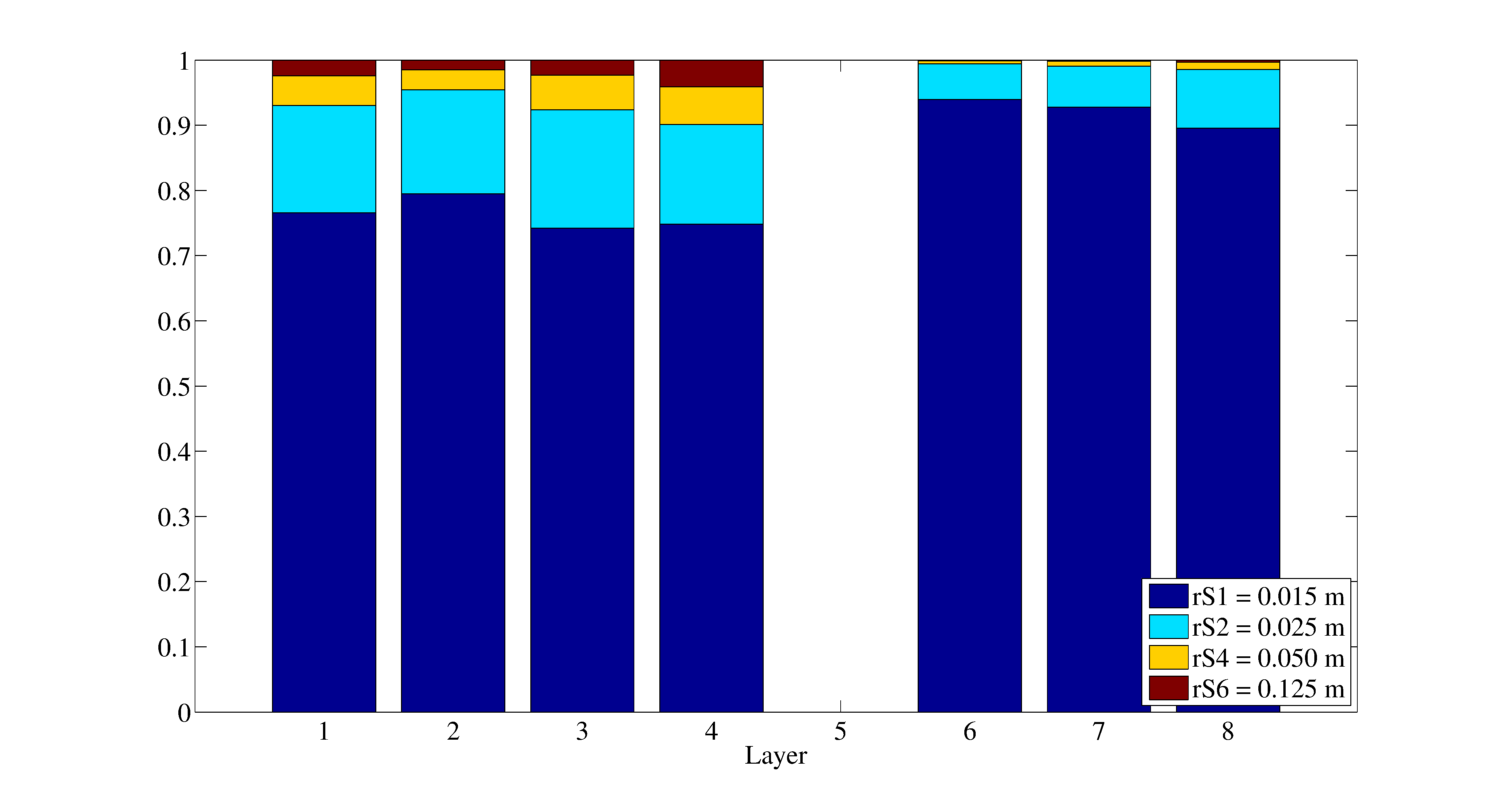
\includegraphics[width=.96\columnwidth]{images/122SinterBarPlot20151123180606}
	  \label{fig:122SinterBarPlot20151123180606}
  }
  \\
  \caption{Sinter bar plot.}
  \label{fig:066sinterbarplot}
\end{figure}

\begin{figure}[!htb]
\centering
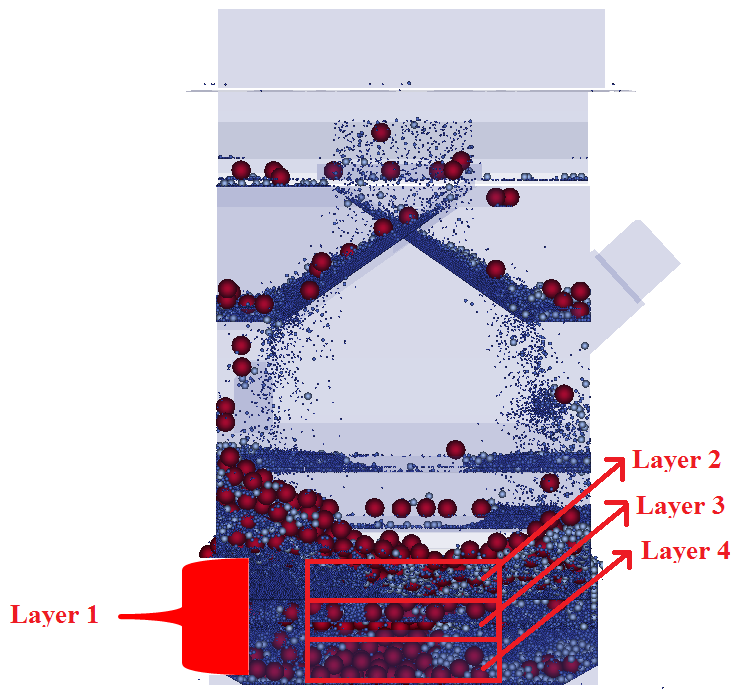
\includegraphics[width=.80\columnwidth]{images/067sinterchute}
\caption[Sinter chute simulation]{Sinter chute simulation.}
\label{fig:067sinterchute}
\end{figure}
\ref{fig:067sinterchute}\\